Functions have a few key points of interest. The first of these are the \emph{intercepts}.

\begin{definition}
    For a function, \(f,\) a point of the form \((x,f(x))\) such that \(f(x) =0\) is called an \emph{\(x\)-intercept}. A point of the form \((0,f(0)\) is called the \emph{\(y\)-intercept}. 
\end{definition}

A function can have no \(x\)-intercepts, \(1\) \(x\)-intercept, or many \(x\)-intercepts. Any function with \(0\) in it's domain has exactly \(1\) \(y\)-intercept. If \(0\) is not in its domain it has no \(y\)-intercepts.

\begin{image}
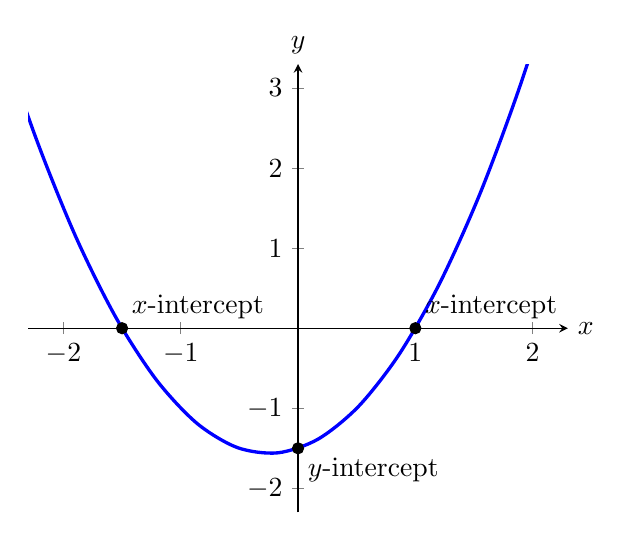
\begin{tikzpicture}
  \begin{axis}[
  xmin=-2.3,
  xmax=2.3,
  ymin=-2.3,
  ymax=3.3,
  axis lines=center,
  xlabel=$x$,
  ylabel=$y$,
  every axis y label/.style=
    {at=(current axis.above origin),anchor=south},
  every axis x label/.style=
    {at=(current axis.right of origin),anchor=west},
  ]
\addplot [very thick, blue,smooth, samples=30] {x^2+x/2-3/2};
\addplot[mark=*] coordinates {(0,-3/2)} node[anchor=north west]{$y$-intercept};
\addplot[mark=*] coordinates {(1,0)} node[anchor=south west]{$x$-intercept};
\addplot[mark=*] coordinates {(-3/2,0)} node[anchor=south west]{$x$-intercept};
\end{axis}
\end{tikzpicture}
\end{image}

These points are named based on the coordinate axis they lie on. That is the \(x\)-intercepts are the points in \(f\) which lie on the \(x\)-axis and the \(y\)-intercepts are the points in \(f\) which lie on the \(y\)-axis.

\desmos{yvaz4pusrf}{100}{600}